% Modelo da UFMG -
% Este modelo foi baseado em: modelo-ufpr.tex,v 1.1 2003/06/30 15:05:18 gweber Exp $
% $Id: modelo-ufpr.tex,v 1.1 2003/06/30 15:05:18 gweber Exp $
%   Licence: LPPL (LaTeX Project Public License)
%     You can change this file in the terms of LPPL
%     (http://www.latex-project.org/lppl.html)
% copyright Rogério C. <rogerioc@cesec.ufpr.br>
%
% ****** DEFINIÇÕES INICIAIS ******	
\documentclass[a4paper,12pt, normaltoc, pnumromarab, pagestart=introducao, tocpage=plain]{abnt}
% Utilize a opção normalfigtabnum para numerar as figuras e tabelas por capítulo
%\usepackage[alf]{abntcite} chamada de referencia alfabetica
\usepackage[num]{abntcite}
\usepackage[brazil]{babel}
\usepackage[utf8]{inputenc}
\usepackage[T1]{fontenc}
\usepackage{indentfirst}
\usepackage{graphicx}														%Package para figuras
\usepackage{float}
\usepackage{geometry}
\geometry{a4paper,left=3cm,right=2cm,top=3cm,bottom=2cm}

%%
%%	Ainda em teste
%%
%\usepackage[bookmarks=false]{hyperref}					%Package para hyper-referências
%\hypersetup{colorlinks,
%							citecolor = black,
%							filecolor = black,
%							linkcolor = black,
%							urlcolor  = blue,
%						pdfnewwindow}
%
% O problema ocorre quando há referências do tipo \cite{} e \citeonline{}
% Há ainda outros problemas -> o figura, antes do número, não altera de cor na lista de figuras.
% O mesmo ocorre na lista de tabelas.
% O sumário aponta para a capa, não para o resumo, lista, apêndices ou anexos correspondentes.
% -> Funciona para capítulos.
%

\makeatletter	%Para que ele entenda o @

% Altera o tamanho das fontes dos capítulos e dos apêndices
\renewcommand{\ABNTchapterfont}{\bfseries}
\renewcommand{\ABNTchaptersize}{\Large}
\renewcommand{\ABNTanapsize}{\Large}

%Altera o espaçamento entre dots
%\renewcommand\@dotsep{2}

%Altera forma de montagem do table of contents
\renewcommand\l@chapter[2]{
  \ifnum \c@tocdepth >\m@ne
    \addpenalty{-\@highpenalty}%
    \vskip 1.0em \@plus\p@
    \setlength\@tempdima{1.5em}%
    \begingroup
      \ifthenelse{\boolean{ABNTpagenumstyle}}
        {\renewcommand{\@pnumwidth}{3.5em}}
        {}
      \parindent \z@ \rightskip \@pnumwidth
      \parfillskip -\@pnumwidth
      \leavevmode \normalsize\ABNTtocchapterfont
      \advance\leftskip\@tempdima
      \hskip -\leftskip
      #1\nobreak\dotfill \nobreak%
      \ifthenelse{\boolean{ABNTpagenumstyle}}
         {%
          \hb@xt@\@pnumwidth{\hss
            \ifthenelse{\not\equal{#2}{}}{{\normalfont p.\thinspace#2}}{}}\par
         }
         {%
          \hb@xt@\@pnumwidth{\hss #2}\par
         }
      \penalty\@highpenalty
    \endgroup
  \fi}

\renewcommand*\l@section{\@dottedtocline{1}{0em}{2.3em}}
\renewcommand*\l@subsection{\@dottedtocline{2}{0em}{3.2em}}
\renewcommand*\l@subsubsection{\@dottedtocline{3}{0em}{4.1em}}

% Cria um comando auxiliar para montagem da lista de figuras
\newcommand{\figfillnum}[1]{%
  {\hspace{1em}\normalfont\dotfill}\nobreak
  \hb@xt@\@pnumwidth{\hfil\normalfont #1}{}\par}

% Cria um comando auxiliar para montagem da lista de tabelas
\newcommand{\tabfillnum}[1]{%
	{\hspace{1em}\normalfont\dotfill}\nobreak
	\hb@xt@\@pnumwidth{\hfil\normalfont #1}{}\par}

% Altera a forma de montagem da lista de figuras
\renewcommand*{\l@figure}[2]{
	\leftskip 3.1em
	\rightskip 1.6em
	\parfillskip -\rightskip
	\parindent 0em
	\@tempdima 2.0em
	\advance\leftskip \@tempdima \null\nobreak\hskip -\leftskip
	{Figura \normalfont #1}\nobreak \figfillnum{#2}}

% Altera a forma de montagem de lista de tabelas
\renewcommand*{\l@table}[2]{
	\leftskip 3.4em
	\rightskip 1.6em
	\parfillskip -\rightskip
	\parindent 0em
	\@tempdima 2.0em
	\advance\leftskip \@tempdima \null\nobreak\hskip -\leftskip
	{Tabela \normalfont #1}\nobreak \tabfillnum{#2}}

% Define os comandos que montam a lista de símbolos
\newcommand{\listadesimbolos}{\pretextualchapter{Lista de Símbolos}\@starttoc{lsb}}
\newcommand{\simbolo}[2]{{\addcontentsline{lsb}{simbolo}{\numberline{#1}{#2}}}#1}
\newcommand{\l@simbolo}[2]{
	\vspace{-0.75cm}
	\leftskip 0em
	\parindent 0em
	\@tempdima 5em
	\advance\leftskip \@tempdima \null\nobreak\hskip -\leftskip
	{\normalfont #1}\hfil\nobreak\par}

% Define o comando que monta a lista de siglas
\newcommand{\listadesiglas}{\pretextualchapter{Lista de Siglas}\@starttoc{lsg}}
\newcommand{\sigla}[2]{{\addcontentsline{lsg}{sigla}{\numberline{#1}{#2}}}#1}
\newcommand{\l@sigla}[2]{
	\vspace{-0.75cm}
	\leftskip 0em
	\parindent 0em
	\@tempdima 5em
	\advance\leftskip \@tempdima \null\nobreak\hskip -\leftskip
	{\normalfont #1}\hfil\nobreak\par}

% Define o tipo de numeração das páginas
%\renewcommand{\chaptertitlepagestyle}{plain}

% Altera a posição da numeração de páginas dos elementos pré-textuais
\renewcommand\pretextualchapter{
	\if@openright\cleardoublepage\else\clearpage\fi
	\pagestyle{\chaptertitlepagestyle}
	\global\@topnum\z@
	\@afterindentfalse
	\@schapter}

% Altera a posição da numeração de páginas dos elementos textuais
\renewcommand{\ABNTsectionmark}[1]{
	\ifthenelse{\boolean{ABNTNextOutOfTOC}}
		{\markboth{\ABNTnextmark}{\ABNTnextmark}}
		{\sectionmark{#1}
		\pagestyle{\chaptertitlepagestyle}}}

% Redefine o tipo de numeração das páginas
\renewcommand{\ABNTBeginOfTextualPart}{
	\renewcommand{\sectiontitlepagestyle}{plainheader}
	\renewcommand{\thepage}{\arabic{page}}
%	\setcounter{page}{1}
}

\makeatother

%Altera o tamanho do parágrafo
\setlength{\parindent}{1.5cm}

% ********************************
% ***** Início do Documento ******
% ********************************
\begin{document}

\begin{titlepage}
\begin{center}
Universidade Federal de Minas Gerais \\
Instituto de Ciências Exatas \\
Departamento de Ciências da Computação \\
\end{center}
\vfill

\begin{center}
%\hspace{.45\textwidth} % posicionando a minipage
\framebox[.8\textwidth][c]{
\begin{minipage}{.7\textwidth}
\begin{center}
\vspace{1cm}
\textbf{TÍTULO DO TRABALHO} \\
\vspace{2em}
por \par
\vspace{2em}
{NOME DO ALUNO} \\
\vspace{2em}
Monografia de Projeto Orientado em Computação I/II \\
\vspace{1em}
\begin{center}
\footnotesize{Apresentado como requisito da disciplina de Projeto Orientado em Computação II do Curso de Bacharelado em Ciência da Computação da UFMG} \\
\end{center}
\vspace{1em}
Prof. Dr. Nome do orientador \\
Orientador
\vspace{1cm}
\end{center}
\end{minipage}
}

\vfill
Belo Horizonte -- MG \\
Ano / [1/2]º semestre
\end{center}
\end{titlepage}



%\sumario

\chapter{INTRODU��O}


\section{Vis�o geral}
A gera��o procedural de modelos � uma �rea da Ci�ncia da Computa��o que prop�e que modelos gr�ficos tridimensionais (representa��o em pol�gonos de algum objeto) possam ser gerados atrav�s de rotinas e algoritmos. Tal t�cnica vem se tornando bastante popular nos �ltimos tempos, tendo em vista que, com o crescimento da ind�stria do entretenimento, h� uma necessidade de se construir modelos cada vez maiores e com um grande n�vel de detalhe. A t�cnica de gera��o procedural vem ent�o como uma alternativa �utiliza��o do trabalho de artistas e modeladores na cria��o de modelos tridimensionais.

O trabalho realizado busca criar um arcabou�o para a gera��o procedural de terrenos, mas que permita tamb�m uma maior 


\section{Objetivo, justificativa e motiva��o}
O objetivo deste trabalho � construir um arcabou�o para a cria��o de terrenos proceduralmente em tempo real e que permita a inser��o de modelos pelo usu�rio. O trabalho pode ser divido em duas vertentes:  visualiza��o de terrenos e a sua gera��o proceduralmente.


O primeiro aspecto (a visualiza��o) � um problema muito estudado no campo da computa��o. O modelo de um terreno � algo que pode demandar um n�mero extremamente alto de tri�ngulos. O processo de gerar a imagem a partir desse modelo (ou renderiza��o) em tempo real fica inviabilizado nos computadores atuais. Faz-se ent�o necess�ria a utiliza��o de t�cnicas que limitam e minimizam o n�mero de tri�ngulos a serem desenhados na tela. Entra a� o uso de \emph{culling} e n�veis de detalhe dos modelos.

A segunda parte, gera��o de terrenos proceduralmente, busca, atrav�s de algoritmos, criar terrenos realistas e que possam ser utilizados em jogos eletr�nicos, simuladores, ou qualquer tipo de aplica��o que necessita de um ambiente virtual tridimensional. Os principais benef�cios dessa gera��o s�o:

\begin{itemize}
	\item Compress�o de dados: todos os modelos s�o criados por algoritmos, e n�o h� a necessidade de se armazenar os dados dos modelos gerados, diminuindo assim o tempo necess�rio para a transmiss�o do conte�do por uma rede, por exemplo.
	\item Conte�do gerado pelo usu�rio de forma f�cil: com a gera��o procedural, o usu�rio n�o precisa de um grande conhecimento ou ent�o a contrata��o de artistas para poder construir modelos 3D. Uma interface amig�vel e alguns ajustes de par�metros s�o o bastante para gerar modelos interessantes.
	\item Produtividade: quanto menor o n�mero de entradas um sistema procedural possuir, menor o trabalho necess�rio para criar modelos.
\end{itemize}

Por�m, um problema recorrente em todos os tipos de gera��o procedural � a falta de controle do usu�rio com o resultado gerado. Quanto mais procedural � um sistema, menos expressivo ele se torna \cite{luke}. Como exemplo, podemos citar programas de modelagem 3D como \emph{Maya} ou \emph{3dMax}: eles oferecem centenas de entradas poss�veis (geometrias representando cones, esferas, etc.), e d�o ao usu�rio o poder de criar praticamente tudo que � imagin�vel \cite{pixar}, resultando em uma alta expressividade; por�m, demandam mais tempo e, como possuem um grande n�mero de entradas, s�o pouco procedurais. J� o jogo \emph{Elite} \cite{elite}, de 1984, cria universos a partir de um �nico n�mero (\emph{seed}); � um exemplo de algo pouco expressivo, mas altamente procedural.

Por isso, o objetivo deste trabalho � tamb�m dar uma maior expressividade � gera��o procedural de terrenos, sem que, no entanto, essa gera��o se torne t�o trabalhosa quanto criar um modelo tridimensional no \emph{Maya} ou \emph{3dMax}.

Em resumo, o trabalho desenvolvido ao longo de POC I e POC II, � um arcabou�o que una a gera��o procedural autom�tica com dados inseridos pelo usu�rio, seja na forma de modelos tridimensionais ou ent�o de mapas de altura (imagens em preto-e-branco que representam algum terreno). Estes dados inseridos pelo usu�rio podem representar �reas de maior interesse para ele, e que necessitam de uma representa��o mais fiel.




\chapter{REFERENCIAL TE�RICO}

V�rios trabalhos publicados abordam a gera��o de modelos tridimensionais com o uso de algoritmos. Alguns destes trabalhos abordam a gera��o de cidades (\cite{parish} e \cite{pseudoinfinite}), outros abordam a gera��o de terrenos realistas (em tempo-real, como os trabalhos \cite{realtime} e \cite{virtual}, ou n�o, como o \emph{MojoWorld} \cite{mojoworld}), ou ent�o a gera��o de �rvores \cite{speedtree}. A principal refer�ncia na �rea � o livro \emph{Texturing and Modeling: A Procedural Approach} \cite{livro}, em que � explicada a gera��o procedural de diversos tipos de modelos.

Algumas t�cnicas largamente utilizadas na gera��o procedural s�o: Sistemas de Lindenmayer (\emph{l-System})\cite{lsystem}, que, atrav�s de uma gram�tica, modela o crescimento de plantas; geometrias fractais \cite{geometrias}; e tamb�m ru�do de Perlin (\emph{Perlin noise} \cite{perlin}). Algumas t�cnicas pertinentes a este trabalho ser�o abordadas na Se��o \ref{terrenos}.

Nas Se��es \ref{grafocenareferencial} e \ref{mapaaltura} ser�o apresentados alguns conceitos relevantes a este trabalho, como Grafo de Cena e Mapa de Altura.


\section{Grafo de cena}
\label{grafocenareferencial}
Um grafo de cena � uma estrutura de dados utilizada em aplica��es gr�ficas e jogos eletr�nicos. O seu objetivo � organizar os objetos presentes em um ambiente virtual (uma cena). Todo os grafos de cena s�o ac�clicos e dirigidos.

No exemplo da Figura \ref{fig:grafocena2}  \cite{grafocena}, o grafo representa uma cena com um carro (\emph{car}) e uma luz (\emph{light}). O nodo {\bf carro} possui, como nodos filhos, quatro {\bf rodas} (\emph{wheel}). A Figura \ref{fig:grafocena1} mostra a cena com o carro e um ponto de luz.

\begin{figure}[H]
	\center{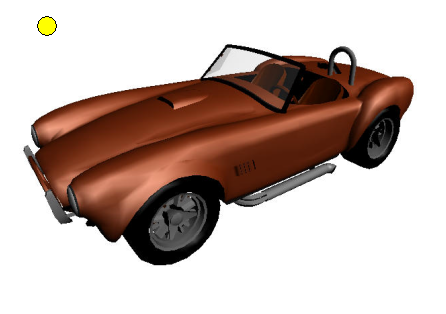
\includegraphics[width=0.25\linewidth]{img/grafocena_exemplo1.png}}
	\caption{\label{fig:grafocena1} Exemplo de uma cena com um carro e um ponto de luz.}
\end{figure}

\begin{figure}[H]
	\center{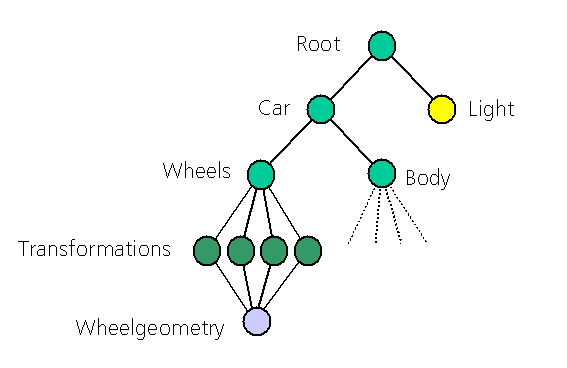
\includegraphics[width=0.35\linewidth]{img/grafocena_exemplo2.png}}
	\caption{\label{fig:grafocena2} Exemplo de um grafo de cena.}
\end{figure}


A maior vantagem de um grafo de cena � a possibilidade de aplicar transforma��es geom�tricas (como rota��o, transla��o, escala) a um nodo, e os filhos desse nodo tamb�m sofrer�o tais transforma��es. T�cnicas mais avan�adas, como desenhar na tela apenas parte de uma cena (ou \emph{culling}), tamb�m podem ser implementadas atrav�s de grafos de cena.


\section{Mapa de altura}
\label{mapaaltura}

Um mapa de altura (ou \emph{heightmap}) � uma imagem bidimensional que armazena dados referentes � altura de um terreno. Geralmente, tons mais claros representam pontos mais altos, enquanto tons mais escuros s�o pontos mais baixos do mapa. A Figura \ref{fig:mapaalturaexemplo} \cite{mapaaltura} � um exemplo de mapa de altura.

\begin{figure}[H]
	\center{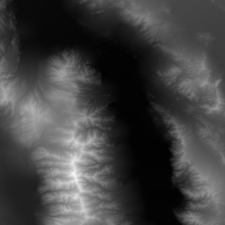
\includegraphics[width=0.20\linewidth]{img/mapaaltura.png}}
	\caption{\label{fig:mapaalturaexemplo} Exemplo de um mapa de altura.}
\end{figure}


\section{Terrenos procedurais}
\label{terrenos}
Existem uma s�rie de t�cnicas para cria��o de terrenos proceduralmente, como ru�do de Perlin e o algoritmo \emph{fractal plasma}, detalhados a seguir.

\subsection{Ru�do de Perlin}
O ru�do de Perlin foi criado pelo Professor Ken Perlin, da \emph{New York University}. O ru�do � usado para simular estruturas naturais, como nuvens, texturas de �rvores, e terrenos.

Para criar um ru�do de Perlin, precisamos de uma fun��o que retorne, para um dado dom�nio, n�meros entre 0 e 1. Para gerarmos esses n�meros, � preciso uma semente (\emph{seed}); dessa forma, em uma segunda execu��o, com uma mesma semente, teremos os mesmos n�meros entre 0 e 1.

A Figura \ref{fig:perlin} \cite{figura_perlin} mostra tr�s fun��es de ru�do, criadas com diferentes valores de amplitude e frequ�ncia. A primeira fun��o poderia ser uma representa��o de montanhas, a segunda de morros, a terceira de blocos de pedras. A quarta fun��o � a soma das tr�s fun��es anteriores. Cada fun��o de ru�do � chamada de um \emph{octave}.

\begin{figure}[H]
	\center{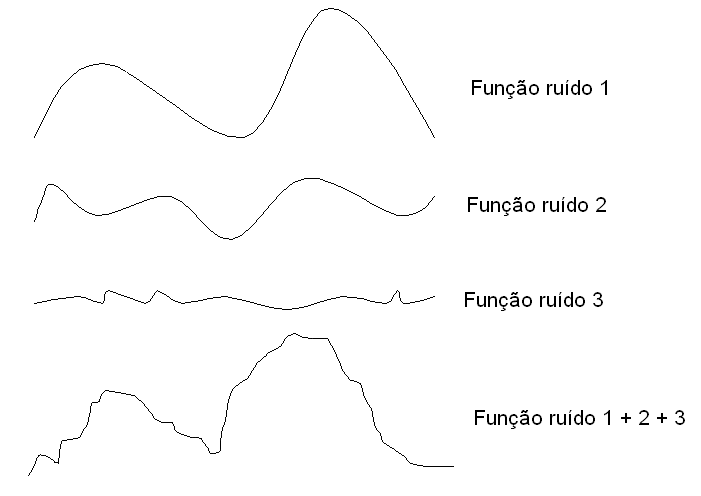
\includegraphics[width=0.5\linewidth]{img/perlin.png}}
	\caption{\label{fig:perlin} Exemplo de um ru�do de Perlin.}
\end{figure}

\subsection{Fractal plasma}
O \emph{fractal plasma} � um outro algoritmo utilizado na gera��o de terrenos. Basicamente, ele inicia com um ret�ngulo onde, na primeira itera��o, cada  aresta recebe um peso aleat�rio, como mostra a Figura \ref{fig:plasma}. Na segunda itera��o, o ret�ngulo � particionado, resultando em quatro ret�ngulos, cujos novos pesos ser�o a m�dia dos pesos das arestas adjacentes, que pode ser acrescido de um pequeno erro. Ao final de um n�mero de itera��es (determinado pelo usu�rio), cada m�dia dos pesos ir� corresponder a uma determinada altura do terreno.

\begin{figure}[H]
	\center{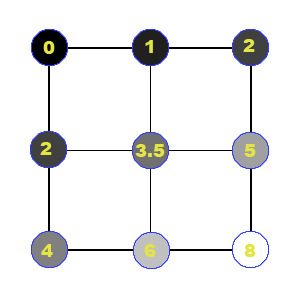
\includegraphics[width=0.25\linewidth]{img/plasma.png}}
	\caption{\label{fig:plasma} Ret�ngulo e seus quatro pontos.}
\end{figure}




\chapter{METODOLOGIA}

\section{Tipo de Pesquisa}
O trabalho proposto � uma pesquisa de natureza aplicada, pois busca aplicar um conhecimento te�rico (t�cnicas de gera��o procedural) e obter um resultado pr�tico na forma de um arcabou�o e tem um  objetivo explorat�rio. A pesquisa se d� em laborat�rio, pois se trata de um ambiente controlado.


\section{Procedimentos metodol�gicos}

O primeiro passo do trabalho foi a escolha de uma \emph{Application Programming Interface} (\sigla{API}{Application Programming Interface}). Por se tratar de uma plataforma aberta e j� estudada em mat�rias durante o curso, o \emph{OpenGL} foi escolhido, juntamente com a linguagem C++. Al�m disso, essa \emph{API} oferece algumas extens�es que permitem maximizar a performance do sistema, como o a estrutura \emph{Vertex Buffer Object} (\sigla{VBO}{Vertex Buffer Object}), que armazena os v�rtices do modelo 3D diretamente na mem�ria da \emph{Graphics Processing Unit} (\sigla{GPU}{Graphics Processing Unit}), diminuindo o n�mero de chamadas para a renderiza��o. O \emph{OpenGL} tamb�m possui algumas bibliotecas, como o \emph{GLFW} \cite{glfw}, para tratamento de eventos do mouse e teclado, o \emph{AntTweakBar} \cite{anttweakbar}, para a constru��o de interfaces gr�ficas e o \emph{DevIL} \cite{devil} para a leitura de imagens.

O desenvolvimento do arcabou�o seguiu t�cnicas de \emph{Programa��o Orientada a Objetos} (\sigla{POO}{Programa��o Orientada a Objetos}), sempre com a inten��o de deixar o sistema o mais flex�vel poss�vel. Um estudo do funcionamento de \emph{frameworks} tamb�m foi necess�rio, envolvendo quest�es como \emph{hot spots}, \emph{frozen spots}, caixa-preta, caixa-branca \cite{framework}.

Foi pesquisado tamb�m diversas t�cnicas procedurais envolvidas na gera��o de terrenos, como, por exemplo, ru�do de Perlin, algoritmo fractal plasma, bem como algumas sistemas que oferecem solu��es ligadas � gera��o procedural, como o \emph{CityEngine} \cite{citygen} e o \emph{MojoWorld} \cite{mojoworld}.

Por fim, foi constru�do um arcabou�o que servir� como base para a implementa��o de algoritmos de gera��o procedural de terrenos, e uma \emph{interface} que permita uma maior intera��o com o usu�rio. Al�m disso, tamb�m foi constru�do um grafo de cena para a organiza��o dos terrenos. Os detalhes ser�o apresentados na pr�xima se��o.



\chapter{RESULTADOS E DISCUSS�O}

Os conhecimentos adquiridos ao longo desse trabalho permitiram a cria��o de um arcabou�o capaz de gerar terrenos procedurais e tamb�m de levar em considera��o algumas entradas do usu�rio. Na Se��o \ref{arcabouco} ser� apresentado tal arcabou�o. Na Se��o \ref{grafocena} ser� mostrado o grafo de cena implementado e, finalmente, na Se��o \ref{terrenosgerados} alguns exemplos de terrenos gerados proceduralmente com o arcabou�o.



\section{Arcabou�o}
\label{arcabouco}

%O arcabou�o implementado aqui teve como um dos principais objetivos a possibilidade de futuras expans�es. A Figura \ref{fig:node} mostra uma hier�rquia de classes implementadas, e que podem ser , como \emph{PerlinNoise} e \emph{Plasma} (para gera��o procedural atrav�s dos algoritmos de ru�do de Perlin e Plasma), e tamb�m a \emph{FileHeightmap}, que � a respons�vel por ler mapas de altura de arquivos de imagem. Quaisquer novos algoritmos de gera��o procedural de terrenos devem ser filhos da classe \emph{Terrain}, que j� encapsula uma s�rie de fun��es pertinentes � visualiza��o de terrenos, como a c�pia dos v�rtices para uma estrutura VBO.

Os m�dulos presentes no arcabou�o t�m como objeto principal possibilitar e facilitar a implementa��o de outras t�cnicas de gera��o procedural de terrenos, sem a necessidade de uma reorganiza��o do arcabou�o. A Figura \ref{fig:arcabouco} mostra um diagrama \emph{Unified Modeling Language} (\sigla{UML}{Unified Modeling Language}) com a organiza��o das principais classes, e uma explica��o de cada m�dulo pode ser vista em seguida.


\begin{figure}[H]
	\center{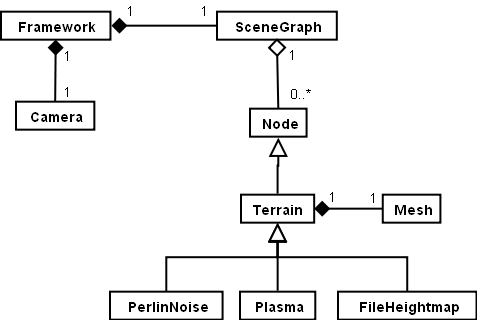
\includegraphics[width=0.5\linewidth]{img/arcabouco.png}}
	\caption{\label{fig:arcabouco} Diagrama UML do arcabou�o.}
\end{figure}

\begin{itemize}
	\item {\bf Framework}: respons�vel por chamar as rotinas de renderiza��o e tamb�m verifica os eventos de entrada do mouse e do teclado.
	\item {\bf Camera}: respons�vel pela movimenta��o no cen�rio.
	\item {\bf SceneGraph}: grafo de cena implementado (e que ser� detalhado na Se��o \ref{grafocena}).
	\item {\bf Node}: classe base para todos os nodos que ser�o inseridos no grafo de cena.
	\item {\bf Mesh}: respons�vel por armazenar os v�rtices da malha do terreno.
\end{itemize}


A c�mera implementada permite que o usu�rio navegue pelo terreno com o controle do mouse e do teclado, padr�o em programas de modelagem 3D, como \emph{Maya} e \emph{3dMax}.

\section{Grafo de cena implementado}
\label{grafocena}

Para a visualiza��o dos terrenos, foi criada uma estrutura de grafo de cena, onde cada nodo representa um terreno gerado (chamado de \emph{patch}). Os \emph{patchs} s�o pequenas partes da geometria do terreno; juntos eles formam o terreno como um todo. A Figura \ref{fig:patch} mostra isso:

\begin{figure}[H]
	\center{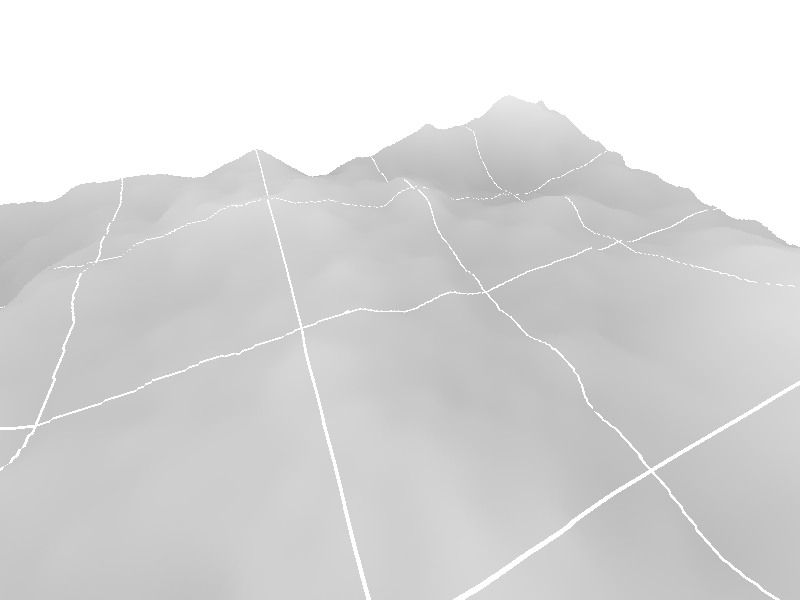
\includegraphics[width=0.4\linewidth]{img/caps/patch.png}}
	\caption{\label{fig:patch} Diversos \emph{patchs} formando um terreno maior.}
\end{figure}

A estrutura leva em considera��o a posi��o atual da c�mera para gerar os terrenos. A Figura \ref{fig:grafo2} considera que a c�mera est� situada acima do {\bf Terreno 0}, e assim ele possui oito nodos filhos ao seu redor.

\begin{figure}[H]
	\center{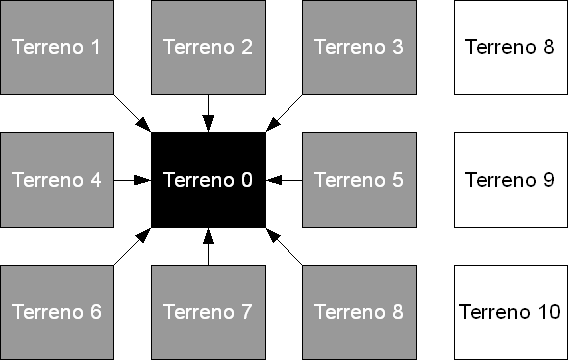
\includegraphics[width=0.4\linewidth]{img/grafo_cena2.png}}
	\caption{\label{fig:grafo2} Grafo de cena e terrenos, com a c�mera no Terreno 0.}
\end{figure}

Na Figura \ref{fig:grafo3}, a c�mera passa a estar em cima do {\bf Terreno 5}. Logo, ser�o gerados os terrenos 8, 9 e 10. Os terrenos 1, 4 e 6 (em branco) poder�o ser exclu�dos, enquanto que os terrenos 0, 2, 3, 7 e 8 passar�o a apontar para um novo nodo pai: o nodo que representa o {\bf Terreno 5}.

\begin{figure}[H]
	\center{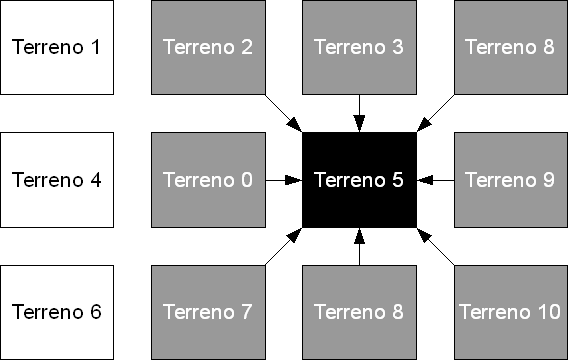
\includegraphics[width=0.4\linewidth]{img/grafo_cena3.png}}
	\caption{\label{fig:grafo3} Grafo de cena e terrenos, com a c�mera no Terreno 5.}
\end{figure}

Outro aspecto levado em considera��o, foi o n�mero de terrenos gerados e o n�mero de terrenos que est�o sendo visualizados. Na Figura \ref{fig:grafo1}, os terrenos em branco foram gerados, mas n�o ser�o renderizados na tela, para economizar recursos da placa de v�deo. O n�mero e as dist�ncias entre os terrenos gerados e visualizados s�o par�metros do arcabou�o.

\begin{figure}[H]
	\center{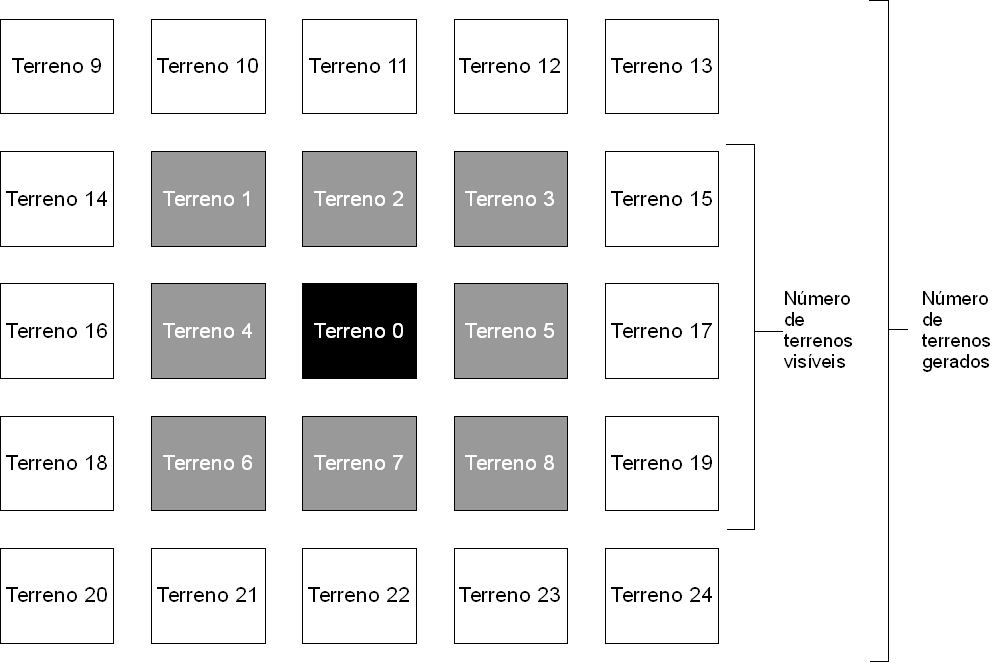
\includegraphics[width=0.6\linewidth]{img/grafo_cena1.png}}
	\caption{\label{fig:grafo1} Visualiza��o e gera��o dos terrenos.}
\end{figure}

\newpage
\section{Terrenos gerados}
\label{terrenosgerados}

A Figuras \ref{fig:tela1} e \ref{fig:tela2} mostram um terreno gerado em um est�gio inicial do arcabou�o.

\begin{figure}[H]
	\center{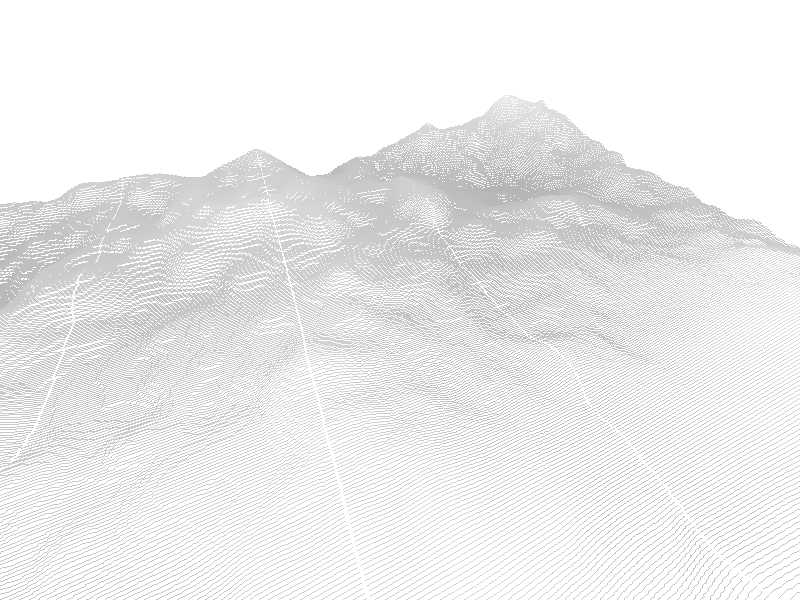
\includegraphics[width=0.7\linewidth]{img/caps/1.png}}
	\caption{\label{fig:tela1} Tela com o terreno gerado (vers�o inicial).}
\end{figure}

As Figuras \ref{fig:tela2}, \ref{fig:tela3} e \ref{fig:tela4} mostram terrenos gerados com uma \emph{interface} provis�ria, onde � poss�vel escolher os par�metros dos terrenos a serem gerados.

\begin{figure}[H]
	\center{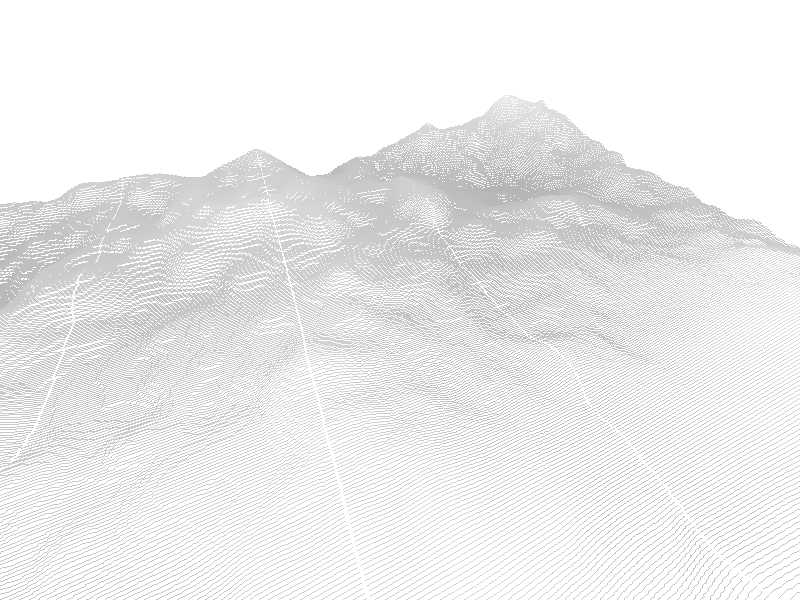
\includegraphics[width=0.7\linewidth]{img/caps/2.png}}
	\caption{\label{fig:tela2} Tela com a \emph{interface} do usu�rio (exibi��o do terreno em \emph{wireframe}).}
\end{figure}

\begin{figure}[H]
	\center{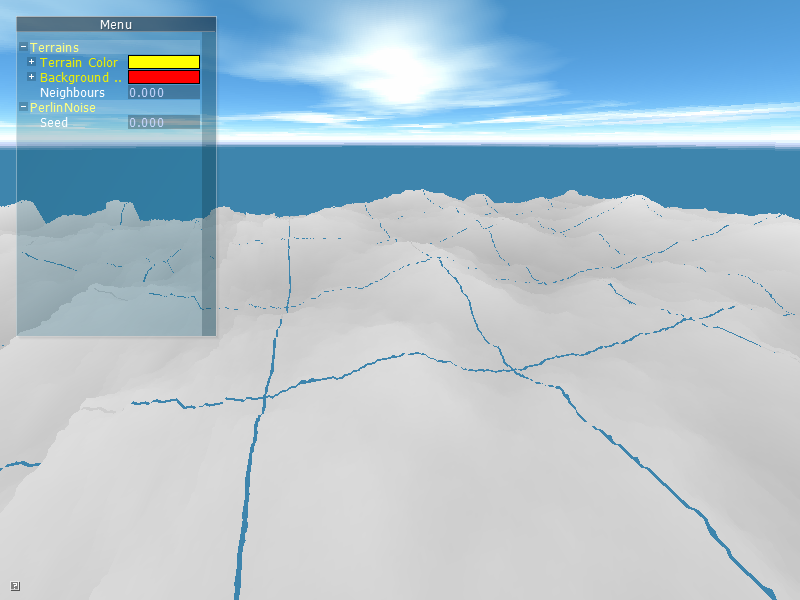
\includegraphics[width=0.8\linewidth]{img/caps/3.png}}
	\caption{\label{fig:tela3} Tela com a \emph{interface} do usu�rio (exibi��o do terreno em tons de cinza).}
\end{figure}

\begin{figure}[H]
	\center{
\includegraphics[width=0.8\linewidth]{img/caps/4.png}}
	\caption{\label{fig:tela4} Tela com a \emph{interface} do usu�rio (exibi��o do terreno com uma textura).}
\end{figure}

\newpage

A Figura \ref{fig:tela5} mostra um terreno gerado proceduralmente e o mapa de altura exibido na Figura \ref{fig:mapaaltura} inserido no arcabou�o (mostrado na Tela em um tom cinza mais escuro, para se destacar do terreno gerado proceduralmente).

\begin{figure}[H]
	\center{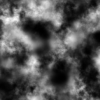
\includegraphics[width=0.25\linewidth]{img/heightmap.png}}
	\caption{\label{fig:mapaaltura} Mapa de altura inserido pelo usu�rio.}
\end{figure}

\begin{figure}[H]
	\center{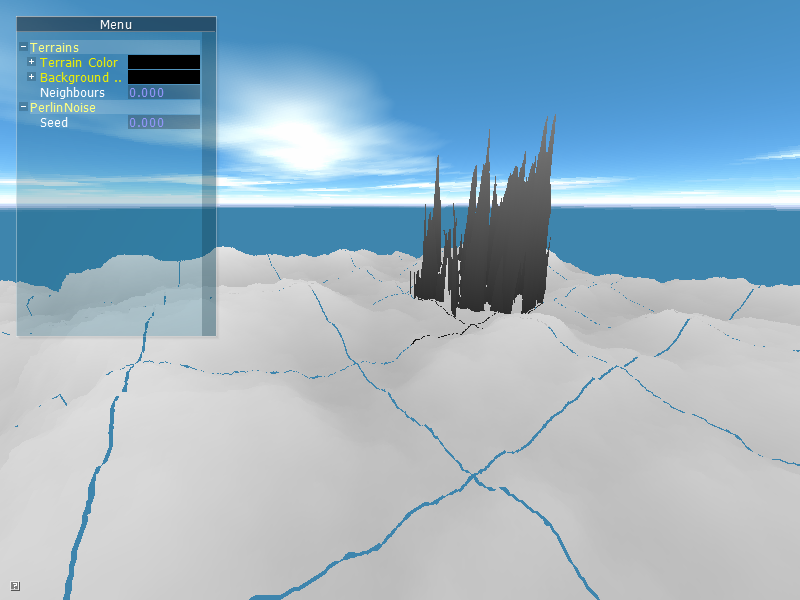
\includegraphics[width=0.8\linewidth]{img/caps/5.png}}
	\caption{\label{fig:tela5} Tela com o terreno gerado e um mapa de altura inserido.}
\end{figure}


\newpage

\section{Testes}
Alguns testes foram feitos para avaliar a varia��o de frames por segundo (\sigla{FPS}{Frames por segundo}) com a altera��o de alguns par�metros e tamb�m o tempo gasto na gera��o procedural. Eles foram executados em um \emph{Athlon64 3500}, com 2GB de mem�ria \emph{RAM} e placa de v�deo \emph{GeForce6600} com 64MB de mem�ria.

A Se��o \ref{teste_geracao} mostra um teste com a gera��o de 100 terrenos proceduralmente.

As Se��es \ref{teste_variando_octaves} e \ref{teste_variando_vizinhos} apresentam testes que consistiam em um v�o da c�mera pelo terreno durante 60 segundos, em um trajeto constante para todos os testes.

\subsection{Teste 1}
\label{teste_geracao}
No primeiro teste, foi medido o tempo gasto com a gera��o de terrenos. Para cada n�mero de \emph{octaves} (4, 16 e 32), foi gerado 100 terrenos, e medido o tempo gasto.

Nas Tabelas \ref{tabela:geracao1} e \ref{tabela:geracao2} � apresentado os tempos das chamadas �s fun��es respons�veis pela gera��o dos terrenos, considerando o algoritmo de ru�do de Perlin. Abaixo uma explica��o sobre cada fun��o:

\begin{itemize}
	\item {\bf FillHeightmap}: Constr�i o terreno, determinando a altura e posi��o de cada v�rtice e armazena em um vetor de \emph{float}. Sua complexidade de tempo � proporcional � largura do terreno (\emph{n}), ao comprimento (\emph{m}) e ao n�mero de \emph{octaves} (\emph{c}). \emph{O(n*m*c)}.
	\item {\bf CopyHeightmap}: Copia o vetor, constru�do na fun��o \emph{FillHeightmap} para um novo vetor VBO. Sua complexidade de tempo � proporcional � largura do terreno (\emph{n}) e ao comprimento (\emph{m}). \emph{O(n*m)}.
	\item {\bf BuildVBOs}: Modifica os ponteiros para o desenho dos vetores VBO. � independente do tamanho do vetor.
\end{itemize}

\begin{table}[H]
	\begin{center}
		\begin{tabular}{|c|c|c|c|c|c|c|}
			\hline
			 - & \multicolumn{3}{|c|}{FillHeightMap} & \multicolumn{3}{|c|}{CopyHeightMap} \\
			\hline
			\emph{Octaves} & \scriptsize M�n. & \scriptsize M�x. & \scriptsize M�dia & \scriptsize M�n. & \scriptsize M�x. & \scriptsize M�dia \\
			\hline
			4 & 0,0410248 & 0,0536568 & 0,0443777 & 0,0737747 & 0,0866761 & 0,0782942 \\
			\hline
			16 & 0,1644840 & 0,2593410 & 0,1698030 & 0,0710867 & 0,0865546 & 0,0734247 \\
			\hline
			32 & 0,3315010 & 0,4503400 & 0,3405685 & 0,0708154 & 0,0778093 & 0,0730120 \\
			\hline
			
		\end{tabular}
		\caption{Tempos da gera��o dos terrenos (em segundos)}
		\label{tabela:geracao1}
	\end{center}
\end{table}

\begin{table}[H]
	\begin{center}
		\begin{tabular}{|c|c|c|c|c|c|c|}
			\hline
			 - & \multicolumn{3}{|c|}{BuildVBOs} & \multicolumn{3}{|c|}{Total}  \\
			\hline
			\emph{Octaves} & \scriptsize M�n. & \scriptsize M�x. & \scriptsize M�dia & \scriptsize M�n. & \scriptsize M�x. & \scriptsize M�dia \\
			\hline
			4 & 0,0078359 & 0,0161562 & 0,0107964 & 0,1264320 & 0,1498800 & 0,1336476 \\
			\hline
			16 & 0,0081773 & 0,0407795 & 0,0114127 & 0,2469740 & 0,3459500 & 0,2550180 \\
			\hline
			32 & 0,0075448 & 0,0129804 & 0,0093645 & 0,4121210 & 0,5310980 & 0,4231183 \\
			\hline
		\end{tabular}
		\caption{Tempos da gera��o dos terrenos (em segundos)}
		\label{tabela:geracao2}
	\end{center}
\end{table}



A Tabela \ref{tabela:geracao3} apresenta os percentuais de tempo de cada chamada da fun��o em rela��o ao tempo m�dio total gasto com a gera��o de um terreno. A Figura \ref{fig:geracao3} mostra um gr�fico com esses dados.

\begin{table}[H]
	\begin{center}
		\begin{tabular}{|c|c|c|c|c|}
			\hline
			\emph{Octaves} & FillHeightMap & CopyHeightMap & BuildVBOs & Total  \\
			\hline
			4 & 32,2\% & 58,6\% & 9,2\% & 100\% \\
			\hline
			16 & 66,6\% & 28,8\% & 4,6\% & 100\% \\
			\hline
			32 & 80,5\% & 17,3\% & 2,2\% & 100\% \\
			\hline
		\end{tabular}
		\caption{Porcentagem dos tempos m�dios de cada chamada, com n�mero vari�vel de \emph{octaves}}
		\label{tabela:geracao3}
	\end{center}
\end{table}


\begin{figure}[H]
	\center{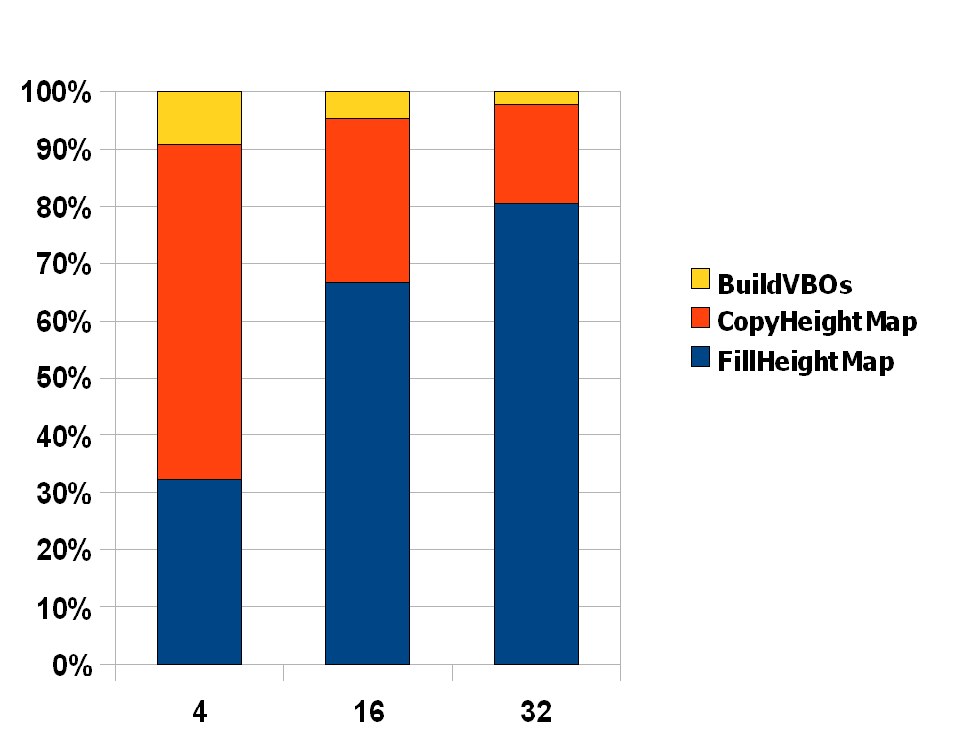
\includegraphics[width=0.5\linewidth]{testes/testes.png}}
	\caption{\label{fig:geracao3} Gr�fico com a porcentagem dos tempos m�dios de cada chamada, com n�mero vari�vel de \emph{octaves}}
\end{figure}

Como podemos observar, o tempo gasto com a c�pia dos dados para a nova estrutura de dados ({\bf CopyHeightMap}) gasta um tempo consider�vel nas tr�s medi��es (com 4, 16 e 32 octaves), algo a ser considerado em trabalhos futuros.

\subsection{Teste 2}
\label{teste_variando_octaves}
O pr�ximo teste (Tabela \ref{tabela:teste1}) mostra o impacto na mudan�a do n�mero de \emph{octaves}, considerando o n�mero de terrenos vizinhos fixo em 2. Quanto maior o n�mero de \emph{octaves}, maior o n�mero de v�rtices da malha do terreno; explicando assim o FPS menor.

Por causa dessa rela��o entre n�mero de \emph{octaves} e n�mero de v�rtices da malha, � poss�vel fazer, em trabalhos futuros, uma gera��o dos terrenos com um n�mero de \emph{octaves} variando de acordo com a dist�ncia da c�mera.


\begin{table}[H]
	\begin{center}
		\begin{tabular}{|c|c|c|c|c|}
			\hline
			 - & \multicolumn{3}{|c|}{\emph{Frames} por segundo} \\
			\hline
			 \emph{Octaves} & \scriptsize M�n. & \scriptsize M�x. & \scriptsize M�dia \\
			\hline
			4 & 17,0 & 75,0 & 38,5 \\
			\hline
			16 & 0 & 73,0 & 25,6 \\
			\hline
			32 & 0 & 73,0 & 19,9 \\
			\hline
		\end{tabular}
		\caption{FPS das execu��es variando o n�mero de \emph{octaves}, e o n�mero de terrenos vizinhos fixo em 2.}
		\label{tabela:teste1}
	\end{center}
\end{table}

%\begin{figure}[H]
	%\center{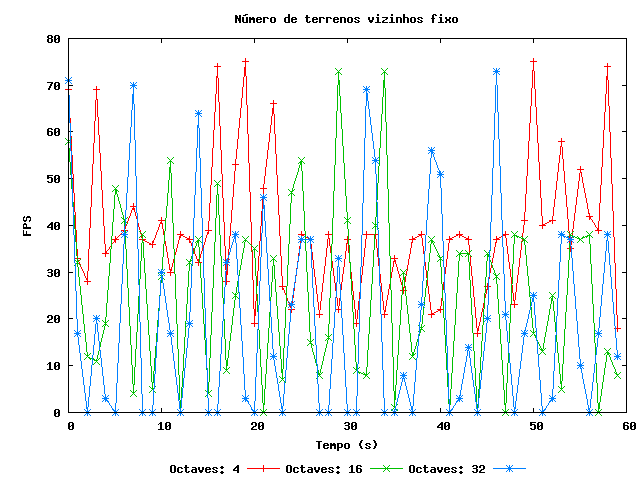
\includegraphics[width=0.8\linewidth]{img/graficos/teste1/teste1.png}}
	%\caption{\label{fig:teste1} Teste variando o n�mero de \emph{octaves}, e o n�mero de terrenos vizinhos fixo em 2.}
%\end{figure}


\subsection{Teste 3}
\label{teste_variando_vizinhos}
O pr�ximo teste (Tabela \ref{tabela:teste2} e Figura \ref{fig:teste2}) mostra o impacto variando o n�mero de terrenos vizinhos.


\begin{figure}[H]
	\center{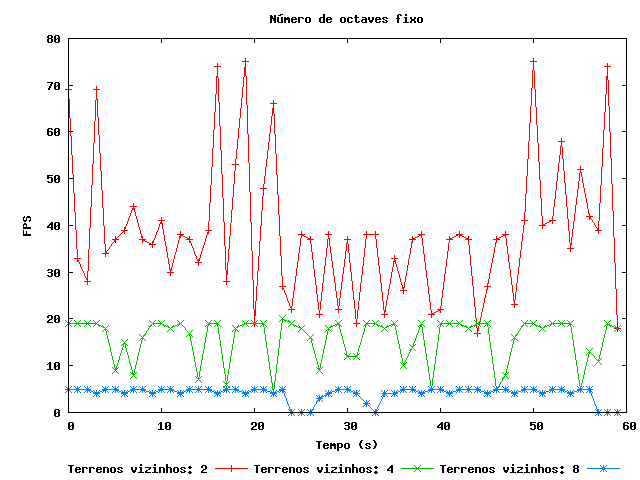
\includegraphics[width=0.8\linewidth]{img/graficos/teste2/teste2.png}}
	\caption{\label{fig:teste2} Teste variando o n�mero de terrenos vizinhos, e o n�mero de octaves fixo.}
\end{figure}

\begin{table}[H]
	\begin{center}
		\begin{tabular}{|c|c|c|c|c|}
			\hline
			 - & \multicolumn{3}{|c|}{\emph{Frames} por segundo} \\
			\hline
			Vizinhos & \scriptsize M�n. & \scriptsize M�x. & \scriptsize M�dia \\
			\hline
			2 & 17,0 & 75,0 & 38,5 \\
			\hline
			4 & 4,0 & 20,0 & 15,8 \\
			\hline
			8 & 0 & 5,0 & 4,1 \\
			\hline
		\end{tabular}
		\caption{FPS das execu��es variando o n�mero de terrenos vizinhos, e o n�mero de octaves fixo.}
		\label{tabela:teste2}
	\end{center}
\end{table}

Como era de se esperar, quanto maior o n�mero de vizinhos, menor o FPS. Para melhorar isso, � poss�vel ajustar o n�mero de vizinhos desenhados de acordo com o computador.



% ********** REFERÊNCIAS **********
%\bibliographystyle{abnt-alf}	 % Existem ainda: abbrv, acm, alpha, amsalpha, amsplain
\nocite{*}
\bibliographystyle{abnt-num}
\bibliography{proposta} % o nome do arquivo .bib com as referências
%\include{bibliografia}															

% \chapter{Entrada de Símbolos e Siglas}
% \par Para fazer a entrada de um símbolo, $\backslash$símbolo\{\simbolo{$\sigma$}{Descrição}\} \{Descriçao\} é a forma % correta. E, para definir uma sigla, $\backslash$sigla\{\sigla{ABNT}{Associação Brasileira de Normas Técnicas}\} % \{Descrição\} deve ser utilizado.
%  \par Obs.: Quando a sigla ou o símbolo aparecerem novamente no texto, não repita o comando, para que a sigla ou símbolo não se repita na lista correspondente.

% *********** APÊNDICES ***********
% ** Condicionados à necessidade **
% \apendice
% \chapter{Primeiro apêndice}
% \par Apêndices são textos elaborados pelo autor a fim de complementar sua argumentação.

% ************ ANEXOS *************
% ** Condicionados à necessidade **
% \anexo
% \chapter{Primeiro anexo}
% \par Anexos são documentos não elaborados pelo autor, que servem de fundamentação, comprovação ou ilustração.

\end{document}

% Quando o número de apêndices ou anexos vier a ser suficiente, é recomendado fazer um sumário separado para os apêndices, localizados imediatamente antes dos apêndices ou anexos. Nesse caso, no sumário principal, apenas é feito referência a este sumário específico.
